\apendice{Especificación de diseño}

\section{Introducción}
En esta parte del anexo definiremos como se han resuelto los objetivos expuestos anteriormente.
\section{Diseño de datos}
El proyecto cuenta con las siguientes entidades:
\begin{itemize}
	\item \textbf{Homogeneous Ensemble}: Es la superclase de los distintos algoritmos que hemos realizado, todos tienen unos parámetros en común que serán los que tiene esta clase abstracta.
	\item \textbf{Disturbing Neighbors}: El método crea características nuevas que se agregarán al conjunto de datos del clasificador base. Dichas características se calculan con el clasificador Nearest Neighbour(NN), construido a partir de unas instancias seleccionadas al azar. Para probar la eficacia utilizamos árboles de decisión como clasificador base. Es un ensemble que esta formado por varios clasificadores base.
	\item \textbf{Random Oracles}: Es un ensemble formado por varios clasificadores base, en el cual, cada clasificador del conjunto se reemplaza por un miniensemble de un par de subclasificadores con un oráculo para elegir entre ellos.
	\item \textbf{Rotation Forest}: Es un ensemble formado por varios clasificadores base, este método genera conjuntos de clasificadores basados en la extracción de características. Crea un conjunto de entrenamiento para un clasificador base, este conjunto se divide al azar en subconjunto. La idea es mejorar la precisión y diversidad dentro del conjunto. La diversidad se basa en la extracción de características para cada clasificador base.
\end{itemize}


\subsection{Diagrama de clases general}\label{diagram-general}
\begin{figure}
\centering
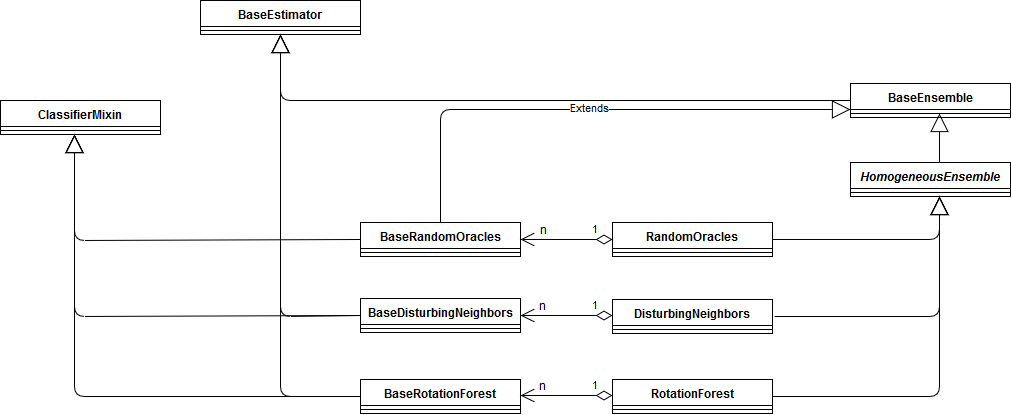
\includegraphics[width=0.95\textwidth]{DiagramGeneral}
\caption{Diagrama de clases general}
\label{fig:DiagramGeneral}
\end{figure}

\subsection{Diagrama de clases implementadas}\label{diagram-implement}
\begin{figure}
\centering
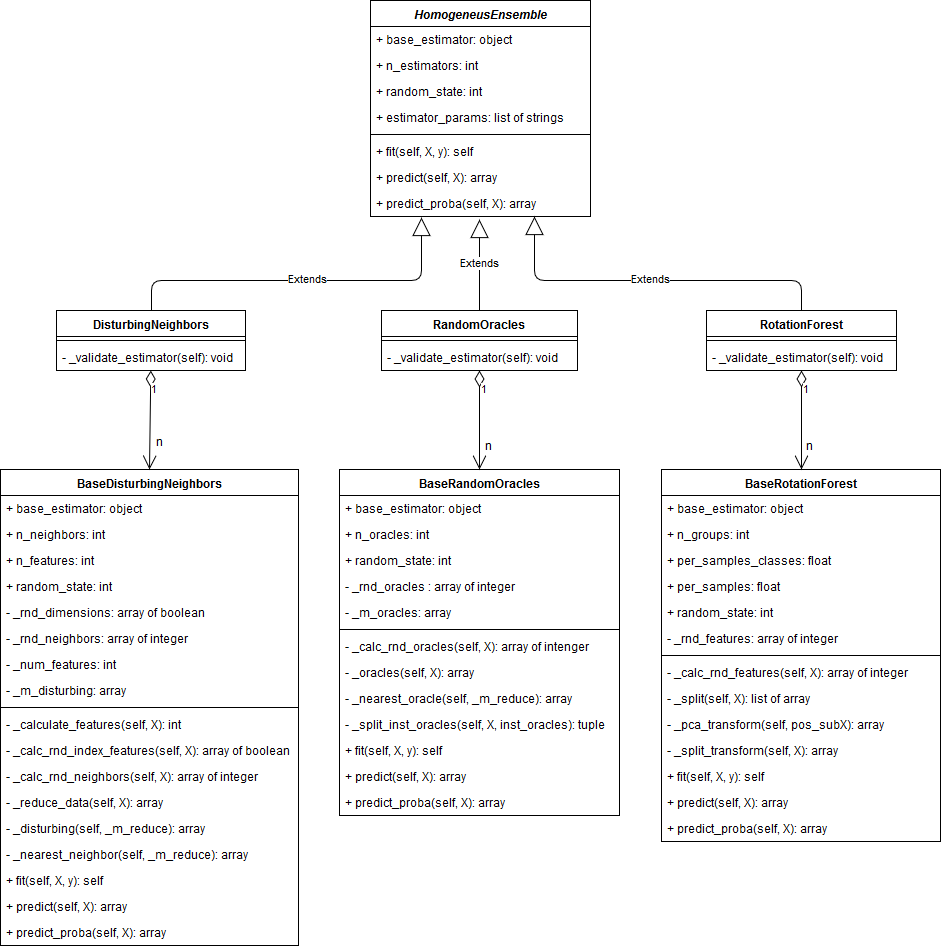
\includegraphics[width=0.95\textwidth]{DiagramImplement}
\caption{Diagrama de clases implementadas}
\label{fig:DiagramImplement}
\end{figure}

\section{Diseño procedimental}
\subsection{Diagrama de secuencias}\label{diagrama-secuencias}
Se ha realizado un diagrama de secuencias de como seria un ejemplo de ejecución del ensemble Disturbing Neighbors, que podemos ver en~\ref{fig:DiagramSequence}.

Los pasos que se han llevado son:
\begin{itemize}
	\item Creamos el clasificador DistubingNeighbors() que a su vez este creara el clasificador base BaseDisturbingNeighbors, y este a su vez DecicisionTreeClassifier.
	\item Una vez creado el clasificador, tendremos tantos clasificadores base como iteraciones tenga nuestro ensemble DisturbingNeighbors. Cada uno de estos clasificadores base entrara el conjunto de datos que le pasamos.
	\item Una vez tengamos nuestros clasificadores base entrenados, lo próximo es hacer la predicción de cada uno de ellos. Que igual que en el entrenamiento se hace sobre cada uno de los clasificadores. Pero lo que al final devolvemos es el promedio de todas las predicciones de los clasificadores base.
	\item Por último realizamos las predicciones de probabilidad, que estas lo que nos devolverán sera la probabilidad de cada una de las clases de que sean 1 o 0. Al igual que en las predicciones, se calcula el promedio de todas. Aunque en la imagen no este no está reflejado, ya que básicamente seria igual que las predicciones. 
\end{itemize}
\begin{figure}
\centering
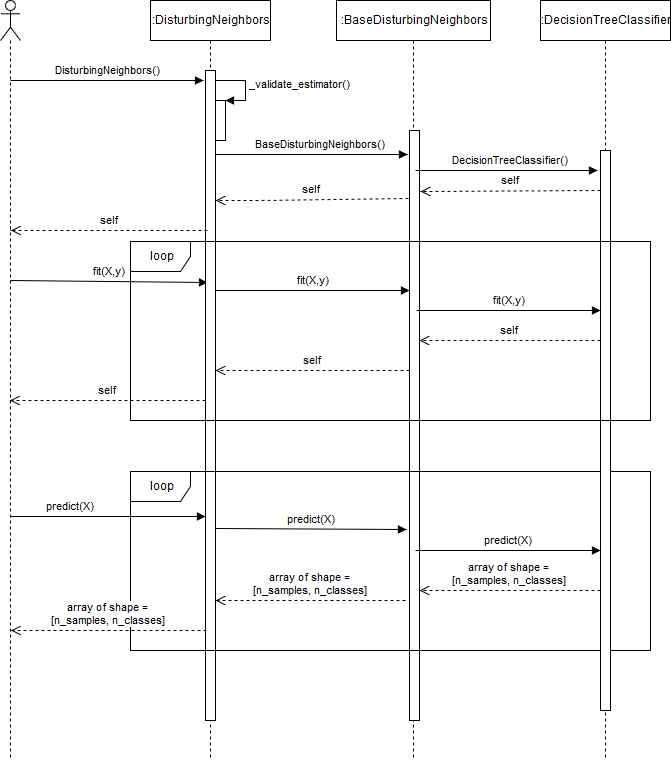
\includegraphics[width=0.95\textwidth]{DiagramSequence}
\caption{Diagrama de secuencias}
\label{fig:DiagramSequence}
\end{figure}

\section{Diseño arquitectónico}
En esta sección, vamos a explicar y mostrar de forma general como esta diseñado el proyecto y como es la distribución de paquetes, que podemos ver en~\ref{fig:DiagramArchitectural}.

Vamos hacer una descripción sobre cada paquete y su contenido.
\begin{itemize}
	\item Src: Aunque no es un paquete en sí, este directorio contiene los notebooks, que son los test para ver los resultados y la eficacia de los algoritmos.
	\begin{itemize}
		\item Sklearn-ubu: Este paquete contendrá todos los ficheros del código fuente de nuestro proyecto, es decir, los clasificadores base y los ensembles.
	\end{itemize}
	\item Sklearn: Aunque este paquete no pertenece a este proyecto, como los algoritmos que hemos realizado, queremos implementarlos en la librería de Scikit-Learn, ha sido necesario hacer usos de este paquete en algunas ocasiones, por ello lo incluimos.
	
\end{itemize}
\begin{figure}
\centering
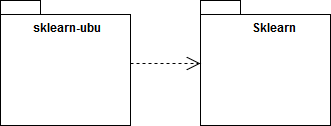
\includegraphics[width=0.95\textwidth]{DiagramArchitectural}
\caption{Diagrama de la estructura}
\label{fig:DiagramArchitectural}
\end{figure}
